% !TEX TS-program = pdflatex
% !TEX encoding = UTF-8 Unicode

\documentclass{beamer}
\usepackage[czech]{babel}
\usepackage[utf8]{inputenc}
\usepackage{times}
\usepackage[T1]{fontenc}
\usepackage{verbatim}
\usepackage{listings}
\usepackage{xcolor}

\mode<presentation>
{
	\usetheme{antibes}
	\usecolortheme{orchid}
}

\setbeamertemplate{navigation symbols}{}

\definecolor{cmtgreen}{RGB}{0,192,0}

\begin{document}

\title{C++; delete Java;}
\subtitle{Část 1: principy OOP v C++}
\author{Kennny}
\date{srpen 2017}

\frame{\titlepage}

\lstset{language=C++,
        basicstyle=\ttfamily,
        keywordstyle=\color{blue}\ttfamily,
        stringstyle=\color{red}\ttfamily,
        commentstyle=\color{cmtgreen}\ttfamily,
        morecomment=[l][\color{magenta}]{\#}
}

\newenvironment{xframe}[1][]
  {\begin{frame}[fragile,environment=xframe,#1]}
  {\end{frame}}

\begin{comment}
\begin{xframe}{tttt}
	\begin{itemize}
		\item
	\end{itemize}
\end{xframe}
\end{comment}



\section{Úvod}
\subsection{O jazyku}


\begin{xframe}{Kurz - motivace}
	\begin{itemize}
		\item základy C++
		\item jazyk C++ je obrovský, všechny jeho funkce a součásti standardní knihovny nelze obsáhnout v jednom malém kurzu
		\item přesun C++ -> Java
		\item zvládnutí KIV/PPR a diplomky bez nějaké větší C++ improvizace
	\end{itemize}
\end{xframe}

\begin{xframe}{Kurz - motivace}
	\begin{figure}
		\centering
		
\includegraphics[width=0.55\textwidth]{newlang.png}
	\end{figure}
\end{xframe}

\begin{xframe}{O jazyku}
	\begin{itemize}
		\item Bjarne Stroustrup, 1983+
		\item Původně rozšíření C
		\item Dialekty\begin{itemize}
			\item C++98 (první oficiální)
			\item C++03
			\item C++11 (pracovně C++0x, pak C++1x)
			\item C++14 (pracovně C++1y)
			\item C++1z (připravovaný, předpokládá se C++17)
			\end{itemize}
	\end{itemize}
\end{xframe}

\begin{xframe}{Navíc proti C}
	\begin{itemize}
		\item OOP (třídy, objekty, dědičnost, polymorfismus, ...)
		\item STL (Standard Template Library)
			\begin{itemize}
				\item string, vector, list, map, set, ...
				\item algorithm, istream/ostream, ...
				\item atd.. atd..
			\end{itemize}
		\item Jiné alokátory (new, delete, delete[])
		\item Výjimky
		\item Šablony
		\item Jmenné prostory
		\item Odlišná sémantika (scope, namespace, ..)
		\item atd.. atd..
	\end{itemize}
\end{xframe}

\begin{xframe}{Jinak proti Javě}
	\begin{itemize}
		\item Není čistě objektový - podporuje kód mimo třídy
		\item Nemá garbagge collector v pravém slova smyslu
		\item Neběží nad virtuálním strojem
		\item Vše je naprosto generické (nemá výjimky, jako třeba syntaxe kolem String v Javě)
		\item Méně bezpečný
		\item A další...
	\end{itemize}
\end{xframe}

\begin{xframe}{Hello world}
\begin{lstlisting}
#include <iostream>

using namespace std;

int main(int argc, char** argv)
{
    cout << "Hello World" << endl;
    return 0;
}
\end{lstlisting}
\end{xframe}

\begin{xframe}{Modern C++}
	\begin{figure}
		\centering
		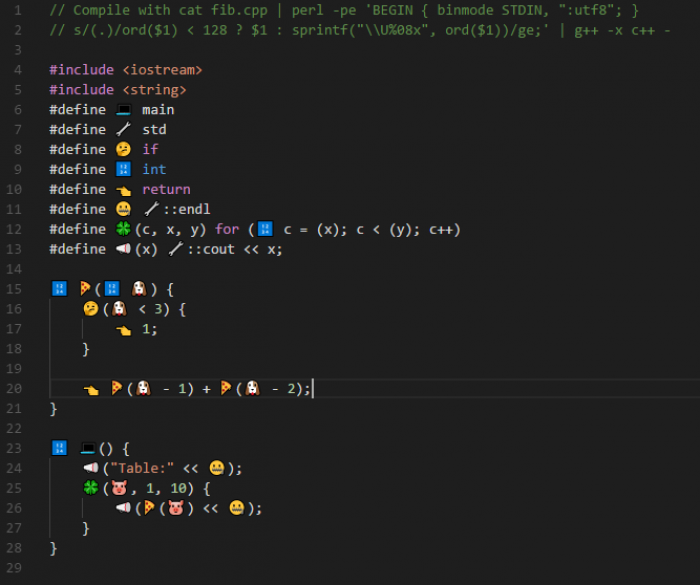
\includegraphics[width=0.75\textwidth]{mcpp.png}
	\end{figure}
\end{xframe}

\section{OOP}
\subsection{Třída}

\begin{xframe}{Třída}
	\begin{itemize}
		\item klíčové slovo \texttt{class}
		\item modifikátory viditelnosti atributů:
			\begin{itemize}
				\item \texttt{public} - viditelný všem
				\item \texttt{protected} - viditelný jen sobě a potomkům
				\item \texttt{private} - viditelný jen sobě
			\end{itemize}
		\item sekce s danou viditelností
		\item konstruktor, destruktor
	\end{itemize}
\end{xframe}

\begin{xframe}{Schéma třídy}
\begin{lstlisting}[basicstyle=\ttfamily\small]
class MyClass
{
    public:
        MyClass();  // konstruktor
        ~MyClass(); // destruktor
        void NejakaMetoda(int parametr);

    protected:
        void ProtectedMetoda();
        int mProtParam;

    private:
        void PrivatniMetoda();
        float mPrivParam;
}
\end{lstlisting}
\end{xframe}

\subsection{Konstruktor, destruktor}

\begin{xframe}{Konstruktor}
	\begin{itemize}
		\item prakticky stejné chování jako v Javě
		\item může jich existovat více, od C++11 lze i "řetězit"~jako v Javě
		\item \emph{member initializer list} - výčet atributů a jejich inicializačních hodnot v momentě volání konstruktoru
\begin{lstlisting}[basicstyle=\ttfamily\small]
MyClass() : mPrivParam(0.0f), mProtParam(10)
{
}
\end{lstlisting}
		\item nepovinné, kromě referencí, ty je nutné inicializovat vždy takto (viz dále)
		\item copy konstruktor - speciální pro kopírování (klonování) objektů
	\end{itemize}
\end{xframe}


\begin{xframe}{Destruktor}
	\begin{itemize}
		\item novinka oproti Javě
		\item volá se v momentě uvolňování objektu z paměti (resp. těsně před dealokací)
		\item explicitně nejvýše jeden
\begin{lstlisting}[basicstyle=\ttfamily\small]
~MyClass()
{
    delete mSomething;
}
\end{lstlisting}
	\end{itemize}
\end{xframe}

\subsection{Definice a implementace}


\begin{xframe}{Definice a implementace}
	\begin{itemize}
		\item lze oddělit definici a implementaci
		\item v hlavičkovém souboru definice
\begin{lstlisting}[basicstyle=\fontsize{8}{9}\selectfont\ttfamily]
class MyClass
{
    public:
        MyClass();
        void NejakaMetoda();
}
\end{lstlisting}
		\item ve zdrojovém souboru implementace 
\begin{lstlisting}[basicstyle=\fontsize{8}{9}\selectfont\ttfamily]
MyClass::MyClass()
{
    //
}

void MyClass::NejakaMetoda()
{
    //
}
\end{lstlisting}
	\end{itemize}
\end{xframe}


\begin{xframe}{Statická a dynamická alokace}
	\begin{itemize}
		\item funguje velmi podobně jako v C
		\item dynamická alokace: \texttt{new} a \texttt{delete} (popř. \texttt{delete[]}) namísto \texttt{malloc} a \texttt{free}
			\begin{itemize}
				\item \texttt{new} volá interně konstruktor třídy
				\item \texttt{delete} destruktor třídy
			\end{itemize}
		\item statická alokace volá konstruktor a destruktor implicitně
		\item snaha využít statickou alokaci a obalit tím alokaci dynamickou (viz dále)
	\end{itemize}
\end{xframe}


\begin{xframe}{Statická a dynamická alokace}
	\begin{itemize}
		\item dynamická alokace objektu
\begin{lstlisting}[basicstyle=\fontsize{9}{10}\selectfont\ttfamily]
MyClass* m = new MyClass(1.0, "parametr konstruktoru");
\end{lstlisting}
		\item statická alokace objektu
\begin{lstlisting}[basicstyle=\fontsize{9}{10}\selectfont\ttfamily]
MyClass m(1.0, "parametr konstruktoru");
\end{lstlisting}

		\item dynamicky alokovaný objekt je nutné ručně uvolnit, statický ne - uvolní se implicitně
	\end{itemize}
\end{xframe}


\begin{xframe}{Scope}
	\begin{itemize}
		\item v kontextu lze přeložit jako "oblast platnosti"
		\item implicitní (vychází z pravidel syntaxe) a explicitní scope
		\item implicitní - např. funkční scope nebo scope \texttt{if}
\begin{lstlisting}[basicstyle=\fontsize{9}{10}\selectfont\ttfamily]
void funkce()
{ // zacatek implicitni scope
    cout << "Nejaka dulezita prace" << endl;
} // konec implicitni scope
\end{lstlisting}
		\item explicitní
\begin{lstlisting}[basicstyle=\fontsize{9}{10}\selectfont\ttfamily]
cout << "Prikaz" << endl;

// zacatek explicitni scope
{
    cout << "Prikaz v explicitni scope" << endl;
} // konec explicitni scope
\end{lstlisting}

	\end{itemize}
\end{xframe}


\begin{xframe}{Scope}
	\begin{itemize}
		\item i v Javě má funkci oblasti platnosti proměnných - jmen, dosažitelnosti, ..
		\item navíc ale po jejím opuštění volá destruktory staticky alokovaných objektů
		
\begin{lstlisting}[basicstyle=\fontsize{9}{10}\selectfont\ttfamily]
void funkce()
{
    cout << "Nejake prikazy, ..." << endl;
    
    MyClass abc(a); // zde se vola konstruktor
    
    cout << "Nejake dalsi prikazy, ..." << endl;
} // zde se vola destruktor abc
\end{lstlisting}
	\end{itemize}
\end{xframe}


\begin{xframe}{Scope}
	\begin{itemize}
		\item často ke scope vážeme tzv. RAII struktury, k těm ale později
		
\begin{lstlisting}[basicstyle=\fontsize{9}{10}\selectfont\ttfamily]
{
    // ziskani mutexu (konstruktor lock_guard)
    std::lock_guard lck(mMutex);

    ...

} // uvolneni mutexu (destruktor)
\end{lstlisting}
	\end{itemize}
\end{xframe}



\begin{xframe}{Příklad}
	\begin{itemize}
		\item Prostor pro příklad 01\_a\_basics
		
		\item Note: \texttt{\#pragma once} je náhražkou bloku:
		
\begin{lstlisting}[basicstyle=\fontsize{9}{10}\selectfont\ttfamily]
#ifndef MUJ_HEADER_H
#define MUJ_HEADER_H

// vlastni obsah hlavickoveho souboru

#endif
\end{lstlisting}
		
	\end{itemize}
\end{xframe}

\subsection{Vlastnosti OOP v C++}


\begin{xframe}{Dědičnost}
	\begin{itemize}
		\item v hlavičce třídy za dvojtečku se uvádí rodičovská třída a viditelnost
		\item viditelnost dědičnosti:
			\begin{itemize}
				\item \texttt{public} - všichni ví o vztahu rodič-potomek
				\item \texttt{protected} - pouze rodič a potomci ví
				\item \texttt{private} - pouze potomek ví
			\end{itemize}
		\item v praxi asi nejčastěji \texttt{public}
		\item v konstruktoru potomka by měl být volán konstruktor rodiče
	\end{itemize}
\end{xframe}

\begin{xframe}{Dědičnost}
\begin{lstlisting}[basicstyle=\fontsize{9}{10}\selectfont\ttfamily]
class Rodic
{
    public:
        Rodic(int a)
        {
            ...
        }
};

class Potomek : public Rodic
{
    public:
        Potomek() : Rodic(5) // volani konstruktoru rodice
        {
            ...
        };
};
\end{lstlisting}
\end{xframe}

\begin{xframe}{Dědičnost a polymorfismus}
	\begin{itemize}
		\item přepisování metod se neděje implicitně
		\item klíčové slovo \texttt{virtual} (rodič)
			\begin{itemize}
				\item bude uvažovat metodu v tabulce virtuálních metod
				\item lze ji tedy přepsat potomkem
			\end{itemize}
		\item klíčové slovo \texttt{override} (potomek)
			\begin{itemize}
				\item není povinné
				\item pouze pro ujištění programátora, že došlo k požadovanému přepisu
			\end{itemize}
	\end{itemize}
\end{xframe}

\begin{xframe}{Polymorfismus - příklad}
\begin{lstlisting}[basicstyle=\fontsize{9}{10}\selectfont\ttfamily]
class Rodic
{
    public:
        virtual void SayHello()
        {
            cout << "Rodic zdravi!" << endl;
        }
};

class Potomek
{
    public:
        virtual void SayHello() override
        {
            cout << "Potomek zdravi!" << endl;
        }
};
\end{lstlisting}
\end{xframe}

\begin{xframe}{Dědičnost a polymorfismus}
	\begin{itemize}
		\item rozdíl nastává v momentě, kdy máme odlišný typ ukazatele/reference, než je objekt na dané adrese
\begin{lstlisting}[basicstyle=\fontsize{9}{10}\selectfont\ttfamily]
Rodic* r = new Potomek();
r->SayHello();
\end{lstlisting}
		\item toto je plně validní, ale jinak se chová s \texttt{virtual} u metod a bez nich
			\begin{itemize}
				\item s \texttt{virtual} - "Potomek zdravi!"
				\item bez \texttt{virtual} - "Rodic zdravi!"
			\end{itemize}
		\item důvodem je (ne)přítomnost v tabulce virtuálních metod
	\end{itemize}
\end{xframe}


\begin{xframe}{Dědičnost a polymorfismus}
	\begin{itemize}
		\item Speciální případ: destruktor
\begin{lstlisting}[basicstyle=\fontsize{9}{10}\selectfont\ttfamily]
virtual ~Rodic();
\end{lstlisting}
		\item rodič by měl mít virtuální destruktor - opět proto, aby se zavolal správný při dealokaci
\begin{lstlisting}[basicstyle=\fontsize{9}{10}\selectfont\ttfamily]
Rodic* r = new Potomek();
r->SayHello();
delete r;
\end{lstlisting}
		\item destruktor je jen speciální metoda
			\begin{itemize}
				\item s \texttt{virtual} - zavolá se destruktor potomka
				\item bez \texttt{virtual} - zavolá se destruktor rodiče
			\end{itemize}
	\end{itemize}
\end{xframe}


\begin{xframe}{Abstraktní třídy}
	\begin{itemize}
		\item abstraktní třída je v C++ vytvořena přítomností tzv. \emph{pure virtual} metody
		\item speciální signatura, metoda nemá implementaci
\begin{lstlisting}[basicstyle=\fontsize{9}{10}\selectfont\ttfamily]
virtual void DoSomething() = 0;
\end{lstlisting}
		\item tato syntaxe ukládá povinnost potomka metodu přepsat
			\begin{itemize}
				\item resp. pokud chceme vytvořit objekt třídy, musí metoda mít někde v hierarchii implementaci
			\end{itemize}
	\end{itemize}
\end{xframe}


\begin{xframe}{Metoda s označením const}
	\begin{itemize}
		\item metody mohou být označeny klíčovým slovem \texttt{const}
		\item znamená to, že nemění stav objektu
\begin{lstlisting}[basicstyle=\fontsize{9}{10}\selectfont\ttfamily]
float GetX() const
{
    return mPositionX;
}
\end{lstlisting}
		\item tyto metody nesmí měnit hodnotu atributů ani ničeho co zaobalují
		\item mohou volat jen jiné metody označené \texttt{const}
	\end{itemize}
\end{xframe}


\begin{xframe}{Přetypování}
	\begin{itemize}
		\item Běžné C-style přetypování
\begin{lstlisting}[basicstyle=\fontsize{9}{10}\selectfont\ttfamily]
Potomek* p = (Potomek*)r;
\end{lstlisting}
			\begin{itemize}
				\item "natvrdo"~ přetypuje
			\end{itemize}
		\item Statické přetypování
\begin{lstlisting}[basicstyle=\fontsize{9}{10}\selectfont\ttfamily]
int* iptr = static_cast<int*>(iptr2);
\end{lstlisting}
			\begin{itemize}
				\item neprovádí kontrolu za běhu, pouze při překladu
			\end{itemize}
		\item Dynamické přetypování
\begin{lstlisting}[basicstyle=\fontsize{9}{10}\selectfont\ttfamily]
Potomek* p = dynamic_cast<Potomek*>(r);
\end{lstlisting}
			\begin{itemize}
				\item provádí kontrolu za běhu
			\end{itemize}
		\item Reinterpretace
\begin{lstlisting}[basicstyle=\fontsize{8}{9}\selectfont\ttfamily]
IPPacket* pkt = reinterpret_cast<IPPacket*>(ether->payload);
\end{lstlisting}
			\begin{itemize}
				\item 1:1 přepis
			\end{itemize}
	\end{itemize}
\end{xframe}


\begin{xframe}{Příklad}
	\begin{itemize}
		\item Prostor pro příklad 01\_b\_inheritance		
	\end{itemize}
\end{xframe}


\begin{xframe}{Vícenásobná dědičnost}
	\begin{itemize}
		\item je možná
		\item ale opatrně, může se vymstít
\begin{lstlisting}[basicstyle=\fontsize{9}{10}\selectfont\ttfamily]
class DvojPotomek : public Otec, public Matka
\end{lstlisting}
		\item dědí metody a atributy obou rodičů
		\item mnohoznačnost je vyřešena uvozením \texttt{Otec::}, popř. \texttt{Matka::}, a to jak u atributů, tak metod
	\end{itemize}
\end{xframe}

\begin{xframe}{Příklad}
	\begin{itemize}
		\item Prostor pro příklad 01\_c\_multiple\_inheritance		
	\end{itemize}
\end{xframe}

\subsection{Operátory}

\begin{xframe}{Operátory}
	\begin{itemize}
		\item C++ dovoluje dodefinovat funkce operátorů
		\item již jsme se setkali s \texttt{<<}
\begin{lstlisting}[basicstyle=\fontsize{9}{10}\selectfont\ttfamily]
cout << "Vypis";
\end{lstlisting}
		\item začneme něčím jednodušším - typický příklad: 2D vektor
			\begin{itemize}
				\item z matematiky víme, že vektory lze sčítat, násobit skalárem, násobit vektorem, ... zde se hodí syntax operátorů
			\end{itemize}
	\end{itemize}
\end{xframe}

\begin{xframe}{Operátory}
	\begin{itemize}
		\item sčítání vektorů = sečtení složek vektorů
		\item uvnitř třídy Vektor:
\begin{lstlisting}[basicstyle=\fontsize{9}{10}\selectfont\ttfamily]
Vektor operator+(const Vektor& second)
{
    return Vektor(x + second.x, y + second.y);
}
\end{lstlisting}
		\item zde zachováváme původní vektory a vytváříme novou instanci
		\item pak lze provést
\begin{lstlisting}[basicstyle=\fontsize{9}{10}\selectfont\ttfamily]
Vektor a(1,2);
Vektor b(2,3);
Vektor c = a + b;
\end{lstlisting}
	\end{itemize}
\end{xframe}


\begin{xframe}{Operátory}
	\begin{itemize}
		\item Operaci lze dodefinovat i vně třídy Vektor:
\begin{lstlisting}[basicstyle=\fontsize{8}{9}\selectfont\ttfamily]
Vektor operator+(const Vektor& first, const Vektor& second)
{
    return Vektor(first.x + second.x, first.y + second.y);
}
\end{lstlisting}
		\item první parametr je levá strana, druhý parametr pravá
	\end{itemize}
\end{xframe}



\begin{xframe}{Operátory}
	\begin{itemize}
		\item takto lze přetížit i operátor bitového posunu
		\item \texttt{std::cout} je globální instance potomka \texttt{std::ostream}
		\item pro výpis vektoru si můžeme přetížit operátor úplně stejně
\begin{lstlisting}[basicstyle=\fontsize{8}{9}\selectfont\ttfamily]
ostream& operator<<(ostream& str, const Vektor& vekt)
{
    return str << "(" << vekt.x << "," << vekt.y << ")";
}
\end{lstlisting}
		\item pak můžeme psát
\begin{lstlisting}[basicstyle=\fontsize{8}{9}\selectfont\ttfamily]
Vektor a(1,10);
cout << a << endl;
\end{lstlisting}
		\item výsledkem bude výpis: \texttt{(1,10)}
	\end{itemize}
\end{xframe}


\begin{xframe}{Příklad}
	\begin{itemize}
		\item Prostor pro příklad 01\_d\_operators
	\end{itemize}
\end{xframe}

\subsection{Pár věcí na závěr}

\begin{xframe}{Další}
	\begin{itemize}
		\item reference = v podstatě kompilátorem řízený pointer, nemůže být \texttt{null}
\begin{lstlisting}[basicstyle=\fontsize{8}{9}\selectfont\ttfamily]
Vektor& refA = a;
\end{lstlisting}
		\item \texttt{nullptr} = typově silná náhrada za \texttt{NULL}
		\item \texttt{final} = třída, kterou nelze dále dědit
\begin{lstlisting}[basicstyle=\fontsize{8}{9}\selectfont\ttfamily]
class Nededitelna final : public Rodic
{
    ...
\end{lstlisting}
	\end{itemize}
\end{xframe}

\begin{xframe}{Namespace}
	\begin{itemize}
		\item jmenný prostor = prostor platnosti objektů a proměnných (a jejich jmen, pochopitelně)
\begin{lstlisting}[basicstyle=\fontsize{8}{9}\selectfont\ttfamily]
namespace Prostor
{
    int promenna;

    class Trida
    {
        ...
    }
}
\end{lstlisting}
		\item dostupná bez instancování, jen je nutné uvodit názvem namespace
\begin{lstlisting}[basicstyle=\fontsize{8}{9}\selectfont\ttfamily]
Prostor::promenna = 10;
\end{lstlisting}
		\item nebo využít \texttt{using}, pak není nutné dále uvozovat
\begin{lstlisting}[basicstyle=\fontsize{8}{9}\selectfont\ttfamily]
using namespace Prostor;
promenna = 10;
\end{lstlisting}
	\end{itemize}
\end{xframe}



\begin{xframe}{Konec 1. části}
\texttt{exit(0);}
\end{xframe}




\end{document}




